\lecture{Cybersecurity}{18~-~11~-~2025}
%
\section{Risk management}
Il risk management è un processo che include:
\begin{itemize}
    \item \textbf{Risk identification} where potential threats are recognized and categorized
    \item \textbf{Risk assessment} evaluates the likelihood and impact of each risk
\end{itemize}
Nel processo di risk management vi è un continuo monitoraggio e tracking di rischi, possibili ``threats'' che possono poi trasformarsi in rischi e vi è l'implementazione di strategie di mitigazione di questi rischi.

%
\subsection{Key components}
%
\paragraph{Services} Something that the ``organization'' must accomplish
%
\paragraph{Asset} Any valuable component that allows the service to perform
%
\paragraph{Vulnerability} Weakness that make the asset vulnerable
%
\paragraph{Menace or threat} Set of action that may cause damage to a service (damaging one or
more assets) exploiting one or more weaknesses
%
\paragraph{Attack} Actual running of a menace
%
\paragraph{Security control} Countermeasure that mitigate/prevent a menace
Notiamo la figura \ref{fig:cybersec_1} a riguardo.

\begin{figure}[h]
    \centering
    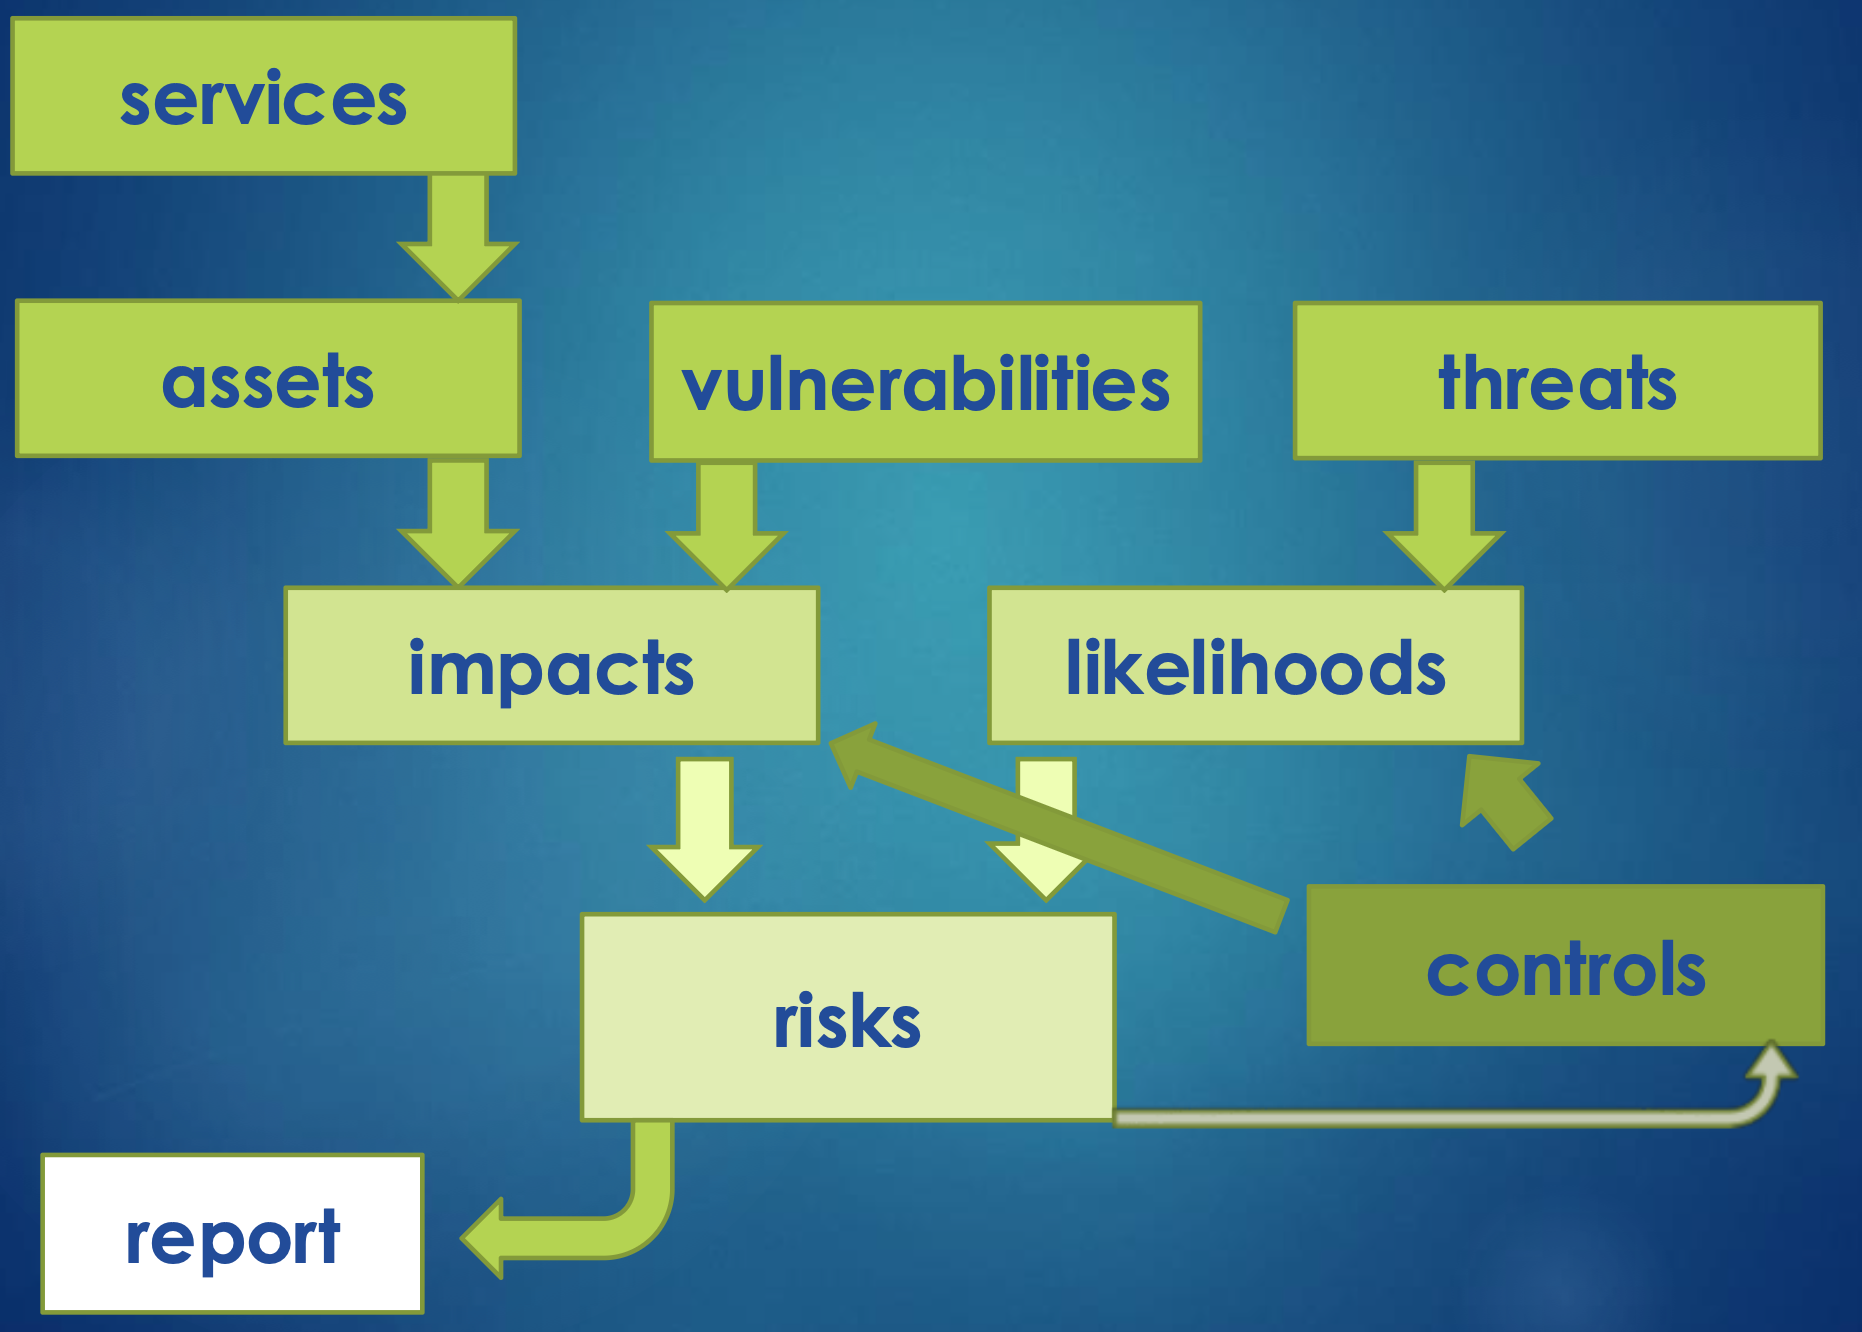
\includegraphics[width=\linewidth]{assets/cybersecurity-1.png}
    \caption{Risk management phases}
    \label{fig:cybersec_1}
\end{figure}

%
\section{Service}
\begin{quote}{Wikipedia}
    Intangible acts or performances whereby the service provider provides value to the customer
\end{quote}
\begin{quote}{Red hat}
    [\dots] a self-contained unit of software functionality, or set of functionalities, designed to complete a specific task such as retrieving specified information or executing an operation.
\end{quote}
Alcuni esempi di servizi sono:
\begin{itemize}
    \item Virtual Reality Car Simulation
    \item Factory Predictive Manufactoring
    \item Authentication Services
    \item \dots
\end{itemize}
%
\subsection{Service Characterizations}
Esistono due principali tipi di servizio:
\begin{itemize}
    \item Business Services, oriented to strategical and organizational goals.
    \item Technical Services, technologies, particularly information and telecommunication ones, to support organizational tasks.
\end{itemize}
%

%
\section{Asset e standardizzazione}
L'identificazione degli asset è il passo cruciale su cui si fonda la protezione. Un asset può essere astratto (\emph{reputazione}), virtuale (\emph{dati}), fisico (\emph{hardware}) o misto (\emph{risorse umane}).
%
\paragraph{Requisiti per l'identificazione (NIST)}
Secondo le specifiche NIST (Interagency Report 7693), un sistema di identificazione deve garantire:
\begin{enumerate}
    \item Unicità: Identificativo univoco e persistente;
    \item Interoperabilità: Standard adottabile da diverse organizzazioni;
    \item Generalità: Capacità di gestire diversi tipi di asset (software, hardware, persone);
    \item Accuratezza: Possibilità di descrivere tutti gli attributi rilevanti.
\end{enumerate}
%
\paragraph{Common Platform Enumeration (CPE)} Mentre il NIST fornisce un modello generale, il CPE è lo standard specifico per identificare classi di applicazioni, sistemi operativi e hardware. È essenziale per l'automazione della sicurezza (es. scansione delle vulnerabilità \dots).

Lo schema CPE v2.3 segue questa struttura:
\begin{lstlisting}[style=CPE]
    cpe:<cpe_version>:<part>:<vendor>:<product>:<version>:<update>:<edition>:<language>:...
\end{lstlisting}

Dove \lstinline[style=CPE]|<part>| indica il tipo: \emph{a} (applicazione), \emph{o} (sistema operativo), \emph{h} (hardware).
Ad esempio: \lstinline[style=CPE]|cpe:2.3:o:microsoft:windows_7:-:-:*:*:home_basic:*:x64:*|

%
\section{Analisi delle vulnerabilità}
Una vulnerabilità è un difetto nel design, nell'implementazione o nella gestione che può essere sfruttato per violare la sicurezza. Per gestire le vulnerabilità in modo sistematico, utilizziamo tre standard principali:
\begin{enumerate}
    \item \emph{CVE (Common Vulnerabilities and Exposures)}: Un elenco/dizionario di vulnerabilità note, ognuna con un ID univoco, descrizione e riferimenti pubblici.
    \item \emph{NVD (National Vulnerability Database)}: Il repository del governo USA che arricchisce i dati CVE con punteggi di gravità e informazioni sulla gestione.
    \item \emph{CWE (Common Weakness Enumeration)}: Una lista comunitaria dei tipi di debolezze software/hardware (es. ``Incorrect Authorization'' \dots). Serve come linguaggio comune per descrivere le cause alla radice.
\end{enumerate}

%
\paragraph{CVSS} Il Common Vulnerability Scoring System (CVSS) fornisce un punteggio numerico che riflette la severità della vulnerabilità. Il punteggio base considera metriche come:
\begin{itemize}
    \item Vettore di Attacco (AV): Rete, Locale, Fisico \dots
    \item Complessità dell'Attacco (AC): Bassa o Alta;
    \item Privilegi Richiesti (PR) e Interazione Utente (UI);
    \item Impatto: Su Confidenzialità, Integrità e Disponibilità.
\end{itemize}

%
\subsection{Threat Landscape}
Le minacce sono cause potenziali di incidenti indesiderati. Secondo il report ENISA, le principali minacce includono:
\begin{itemize}
    \item \emph{Malware}: Include virus, trojan, spyware e information stealers;
    \item \emph{Ransomware}: Un tipo di malware che blocca dei dati/portali e richiede un riscatto. Tattiche recenti includono la ``doppia estorsione'' (furto dati prima della cifratura);
    \item \emph{Social Engineering}: Manipolazione psicologica (es. Phishing) per ottenere accessi o dati;
    \item \emph{Supply Chain Attacks}: Compromettere un fornitore per colpire i clienti a valle.
\end{itemize}

%
\subsection{Agenti di minaccia}
Chi attacca? Si spazia da attori supportati dagli stati (cyberwarfare), al crimine organizzato, fino agli hacktivisti. Le motivazioni seguono l'acronimo MICE:
\begin{itemize}
    \item Money (Denaro): Guadagno diretto o indiretto;
    \item Ideology (Ideologia): Politica, religiosa o attivismo;
    \item Coercion (Coercizione): Ricatto;
    \item Ego (Ego): Reputazione o sfida personale.
\end{itemize}

%
\section{Modellazione del Rischio e Strategie di Mitigazione}
Il rischio comporta perdite che possono essere monetarie, strategiche (reputazione), legali o di sicurezza fisica.
%
\paragraph{Analisi costi-benefici} Per decidere se applicare una contromisura, si usa la logica del trade-off. Una misura di sicurezza è valida se il risparmio generato è maggiore del suo costo. Formula semplificata del risparmio:
\[
    \text{Savings} = RC \times I - CC
\]
dove:
\begin{itemize}
    \item \emph{RC} (Risk Cost): Costo del rischio (es. Annual Loss Expectancy (ALE));
    \item \emph{CC} (Countermeasure Cost): Costo della contromisura;
    \item \emph{I} (Influence): Efficacia della contromisura (copertura).
\end{itemize}

%
\paragraph{Le 4 Strategie di Gestione}
Una volta valutato, il rischio può essere gestito in quattro modi:
\begin{enumerate}
    \item Retention (Accettazione): Accettare il rischio e le relative conseguenze;
    \item Avoidance (Evitamento): Decidere di non intraprendere l'attività rischiosa;
    \item Reduction (Riduzione): Applicare controlli per diminuire probabilità o impatto;
    \item Transfer (Trasferimento): Condividere il rischio con terzi (es. assicurazione).
\end{enumerate}

%
\section{Controlli di Sicurezza}
I controlli di sicurezza servono a proteggere la triade \emph{CIA} (Confidenzialità, Integrità, Disponibilità). Lo standard ``NIST SP800~-~53'' definisce 20 famiglie di controlli, di seguito vediamo solo le più importanti:
\begin{itemize}
    \item AC (Access Control): Gestione account, principio del privilegio minimo (es. AC-2, AC-6);
    \item AT (Awareness and Training): Formazione contro il phishing e literacy di sicurezza (es. AT-2);
    \item AU (Audit and Accountability): Log degli eventi e revisione per tracciare attività anomale (es. AU-2, AU-6);
    \item CM (Configuration Management): Baseline di configurazione e controllo delle modifiche (es. CM-2, CM-3);
    \item IA (Identification and Authentication): Verifica dell'identità di utenti e dispositivi, inclusa la MFA (es. IA-2);
    \item IR (Incident Response): Piani, test e training per rispondere agli incidenti (es. IR-2, IR-3);
    \item PE (Physical Protection): Accesso fisico agli edifici e controllo visitatori (es. PE-2);
    \item SC (System and Communications Protection): Protezione dei confini (firewall) e crittografia (es. SC-7, SC-13);
    \item SI (System and Information Integrity): Gestione patch e protezione da codice malevolo (es. SI-2, SI-3);
    \item SR (Supply Chain Risk Management): Valutazione dei fornitori esterni (es. SR-5).
\end{itemize}